\chapter{Sigue personas}
\label{cap:capitulo5}
Ahora que ya tenemos integrado ROS2 dentro de la plataforma de VisualCircuit, vamos a crear varios proyectos usando los bloques drivers que hemos creado.
El primero de ellos será un comportamiento de \textit{follow-person} usando reconocimiento visual.

\section{Desarrollo inicial sigue-personas}
\label{sec:VC_intro}

En primer lugar, debemos preparar el entorno de pruebas, por lo que aprovecharemos un modelo de persona teleoperada que creó Carlos
Caminero\footnote{\url{https://github.com/RoboticsLabURJC/2021-tfg-carlos-caminero/tree/main/amazon_hospital/hospital_world}}, compañero de la carrera.

\begin{figure} [H]
    \begin{center}
        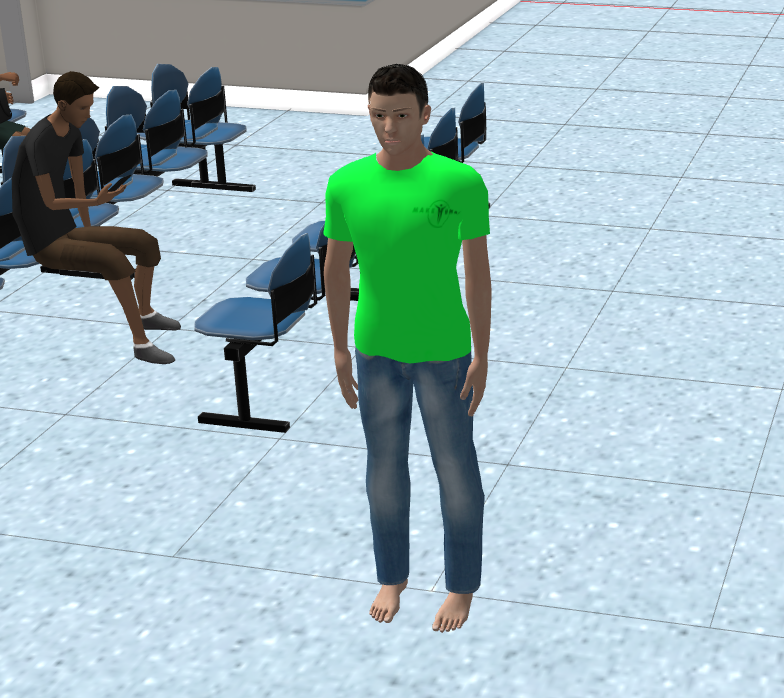
\includegraphics[width=7cm]{figs/c5/elman.png}
    \end{center}
    \caption[Modelo de persona en gazebo]{Modelo de persona teleoperable en gazebo.}
    \label{fig:teleop_person}
\end{figure}
El mundo que tenía Carlos creado incluía muchos elementos del entorno que no son necesarios en nuestro caso, por lo que modificaremos el
mundo para dejar únicamente al robot y a la persona. El modelo del robot que usaremos será el que mencionamos en el capítulo \ref{subsec:turtlebot2_sim},
ya que incluye tanto cámara como láser.\\

El comportamiento sigue-persona que buscamos desarrollar con VisualCircuit consiste en rotar en círculos hasta encontrar a una persona mediante
algoritmos de detección visual de objetos y mantener a la persona centrada en la imagen, al igual que mantenernos a una distancia constante,
usando así la función de lectura de distancias de la cámara. Por ello sólamente la cámara como sensor, ya que esta función mencionada nos permite no
usar el láser y evitar un código más complejo.\\

\begin{figure} [H]
    \begin{center}
        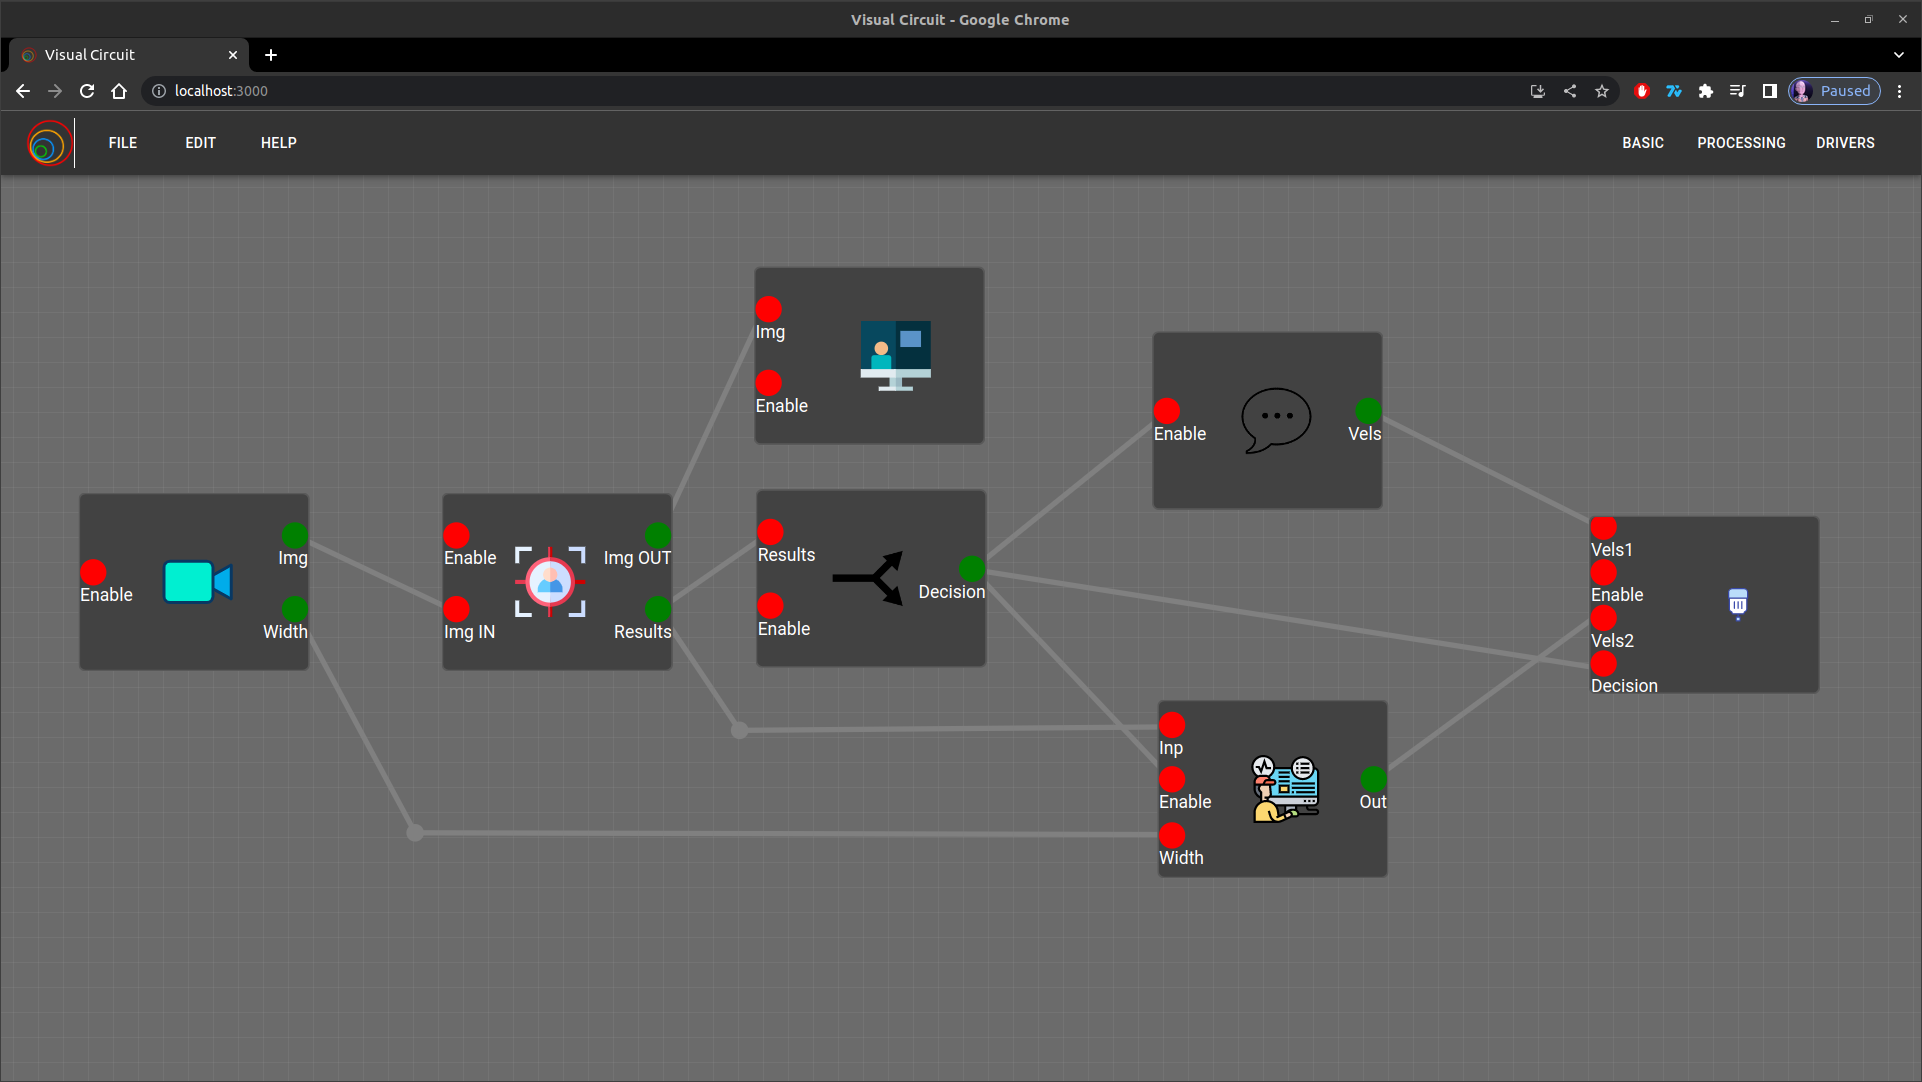
\includegraphics[width=12cm]{figs/c5/follow_person_initial.png}
    \end{center}
    \caption[Circuito sigue-personas inicial]{Circuito inicial del algoritmo sigue-persona.}
    \label{fig:initial_follow_person}
\end{figure}

La lógica que seguirá será la siguiente: recibir la imagen del \textit{topic} de la cámara y compartirla con el bloque de detección de objetos,
enviar la imagen con las detecciones al bloque \textit{screen} para visualizar en tiempo real lo que está analizando el robot,
y también mandaremos los resultados a un bloque que decidirá qué hacer. Este bloque activa un PID en caso de que haya una persona en la imagen,
o el comportamiento de rotación en caso de que no se haya encontrado ninguna.
En ambos casos, se envía la decisión a los bloques que generan las velocidades y también al bloque \textit{MotorDriver} que hemos creado en
el punto \ref{sec:drivers_creacion}, que recibe tanto las distintas velocidades, como la decisión que se ha tomado, y envía al \textit{topic} la adecuada.

La detección visual utiliza yolov3\footnote{\textbf{YouOnlyLookOnce (YOLO)}: \url{https://pjreddie.com/darknet/yolo/}},
un algoritmo de detección de objetos a tiempo real que permite identificarlos tanto en video como en imágenes usando redes neuronales
(darknet\footnote{\textbf{DarkNet}: \url{https://pjreddie.com/darknet/}}). El bloque que ya está integrado en VisualCircuit nos sirve para nuestra aplicación,
pero he tenido que modificarlo para poder extraer también la localización de la \textit{Bounding Box} que corresponde a la persona y compartirla con otros bloques.\\

Para ello, después de obtener los nombres de los objetos encontrados, recorremos toda la lista comprobando si hay alguna persona,
en caso de haberla enviamos la \textit{Bounding Box} correspondiente, sino, enviamos un \textit{array} con cuatro valores ``-1'' para indicar que está vacío.

\begin{code}[H]
    \begin{lstlisting}[language=python]
    #**********
        #forward Pass
        results = net.forward(outputNames)
        findObjects(results,frame)
        is_person = False
        for i in classIds:
            if(className[i] == "person"):
                is_person = True
                break
        to_send = [-1,-1,-1,-1]
        if(is_person):
            to__send = bbox[i]
        outputs.share_image("Img OUT", frame)
        outputs.share_array("Results", to__send)
        synchronise()
    #**********
    \end{lstlisting}
    \caption[Modificación al bloque detector de objetos]{Modificación al bloque de la detección de objetos.}
    \label{cod:mod_object_detector}
\end{code}

El siguiente bloque (\ref{cod:decision_follow_person}) es el que toma las decisiones de qué comportamiento seguir.
Para ello, primero esperaremos hasta recibir algún resultado de la visión y así no movernos antes haber podido analizar la situación.\\
Una vez que tengamos resultados, miraremos si es una \textit{Bounding Box} válida, en caso de serlo, la decisión será seguir lo que indique el bloque PID.
En caso de ser una caja vacía (\textit{array} de ``-1'') activaremos un contador para aplicar un filtro de paso bajo.\\
Este filtro nos permite evitar cambiar de comportamiento por pequeños errores en la detección de objetos.
Está establecido a 10, por lo que al llegar a 10 imágenes seguidas sin una persona en la imágen, cambiaremos de comportamiento al de la rotación.\\

\begin{code}[H]
    \begin{lstlisting}[language=python]
        def main(inputs, outputs, parameters, synchronise):
            auto_enable = True
            try:
                enable = inputs.read_number("Enable")
            except Exception:
                auto_enable = True
             
            while(True):
            # Wait for results
                results = inputs.read_array("Results")
                try:
                    if(results.any()):
                        break
                except Exception:
                    continue
    
            not_to_enable = 0
            to_enable = 1
            lowpass_filter = 10
            counter = 0
            print("EMPEZAMOS")

            while(auto_enable or inputs.read_number('Enable')):
                results = inputs.read_array("Results")
                if(results[0] != -1):
                    # Follow
                    counter = 0
                    outputs.share_number("Decision", 1)
                elif(counter < lowpass_filter):
                    # Follow but low-pass filter
                    counter += 1
                    outputs.share_number("Decision", 2)
                else:
                    # Rotation
                    outputs.share_number("Decision", 0)
    \end{lstlisting}
    \caption[Código bloque decisión sigue-persona]{Código del bloque de decisiones del sigue-persona.}
    \label{cod:decision_follow_person}
\end{code}

En cuanto al bloque que envía la velocidad correspondiente al comportamiento de rotación, tiene un bucle que lee el cable que le llega, en caso de ser un "1" (\textit{True}) informa en la terminal que estamos rotando y envía una velocidad angular de 1rad/s para el eje Z.

\begin{code}[H]
    \begin{lstlisting}[language=python]
    import numpy as np

    def main(inputs, outputs, parameters, synchronise):
        try:
            while 1:
                if(inputs.read_number('Enable')):
                    print("ROT")
                    vels = [0,0,0,0,0,1]
                    to_write = np.array(vels, dtype='<U64')
                    outputs.share_array("Vels", to_write)   
                    synchronise()
        except Exception as e:
            print("Error")
    \end{lstlisting}
    \caption[Código bloque rotación sigue-persona]{Código del bloque de la rotación del sigue-persona.}
    \label{cod:rotation_follow_person}
\end{code}

En paralelo al anterior, también se puede activar el bloque PID\footnote{\textbf{PID}: Controlador proporciona, integral y derivativo.}. Su estructura consiste en tres entradas (Resultados de la detección de objetos, ancho de la imagen y \textit{enable}), tres parámetros para las tres constantes del controlador y una salida para la velocidad lineal y angular final que aplicaremos al robot.

\begin{figure} [H]
    \begin{center}
        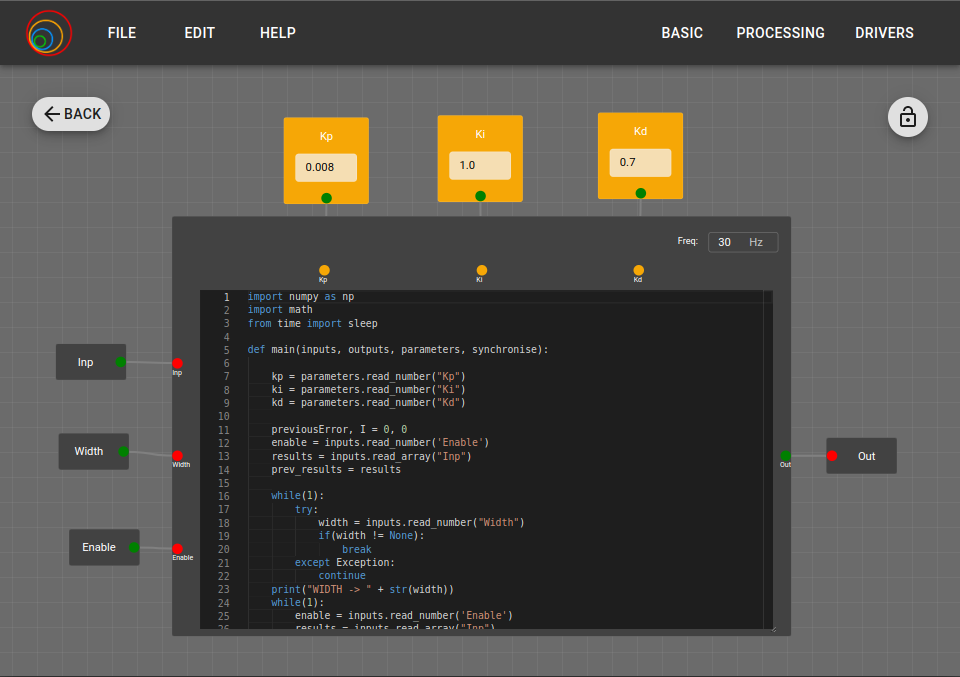
\includegraphics[width=10cm]{figs/c5/PID_follow_person.png}
    \end{center}
    \caption[Circuito del bloque PID sigue-persona]{Circuito del bloque PID del sigue-persona en VisualCircuit.}
    \label{fig:initial_follow_person}
\end{figure}

Analizando el código del bloque PID, podemos ver que 

\begin{code}[H]
    \begin{lstlisting}[language=python]
    import numpy as np
    import math
    from time import sleep

    def main(inputs, outputs, parameters, synchronise):

        kp = parameters.read_number("Kp")
        ki = parameters.read_number("Ki")
        kd = parameters.read_number("Kd")

        previousError, I = 0, 0
        enable = inputs.read_number('Enable')
        results = inputs.read_array("Inp")
        prev_results = results

        while(1):
            try:
                width = inputs.read_number("Width")
                if(width != None):
                    break
            except Exception:
                continue
        while(1):
            enable = inputs.read_number('Enable')
            results = inputs.read_array("Inp")
            if(enable != 0):
                try:

                    if(enable == 1):
                        error = float(results[0]+results[2]/2) - width/2
                        prev_results = results
                    else:
                        error = float(prev_results[0]+prev_results[2]/2) - width/2
                    sleep(0.01)

                    P = error
                    D = error - previousError
                    PIDvalue = (kp*P)  + (kd*D)
                    previousError = error

                    linear_velocity = 0.0
                    angular_velocity = -PIDvalue

                    data = [linear_velocity, 0,0,0,0, angular_velocity]
                    outputs.share_array("Out", data)

                    synchronise()
                except Exception:
                    synchronise()
                    continue
    \end{lstlisting}
    \caption[Código bloque PID sigue-persona]{Código del bloque del PID sigue-persona.}
    \label{cod:PID_follow_person}
\end{code}
































\newpage
\begin{figure} [H]
    \begin{center}
        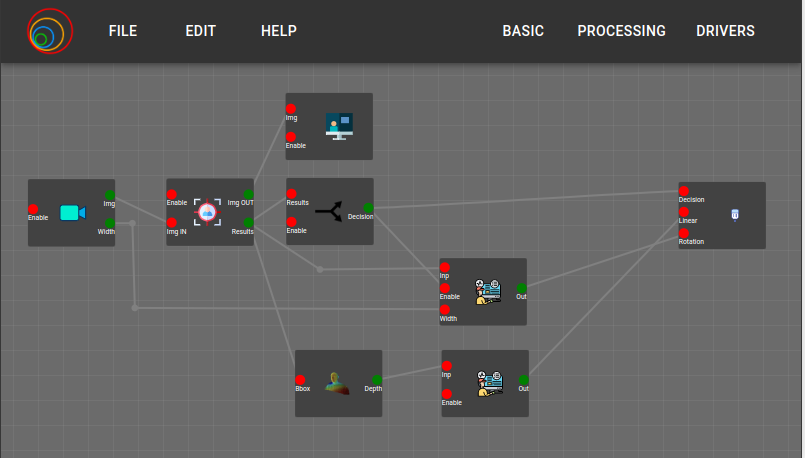
\includegraphics[width=12cm]{figs/c5/follow_person_final_model.png}
    \end{center}
    \caption[Circuito sigue-personas inicial]{Circuito inicial del algoritmo sigue-persona.}
    \label{fig:initial_follow_person}
\end{figure}







